\chapter{Scope}
\section{Aim and Hypothesis}
The development of a physically informed spectral analysis framework for quantifying Antarctic subglacial landscape characteristics and classifying bed morphology into archetypes for ice sheet modelling.

We propose that to identify subglacial landscape class it is necessary to have multiple measured statistics. A radar echo sounding (RES) transect bounds the class rather than pinpointing it. Our scheme uses a vector whose elements are either used as "classifiers" or "descriptors" to match RES transects into landscape archetypes defined from the literature. Beds usually fit more than one label and the classifiers typically leave 2, descriptors check whether a surviving label is covering measurably different beds. Our transect analysis scheme recovers bed texture directly along the radar profile, where bed texture 50~km apart decorrelates. By contrast, current continent-wide gridded products such as Bedmap3 is posted at 500~m, but 93\% of its ice-thickness cells are interpolated between flight lines~\cite{Pritchard_2025}, so texture at these scales is inferred rather than measured.

\section{Objectives}
\begin{itemize}
    \item{\textbf{Derive a landscape classification vector}} based on spectral and morphometric elements 
        \\\textbf{Classifiers}
        \begin{enumerate}
            \item{\texttt{$\beta$}}: power-law exponent of the elevation PSD,
            \item{\texttt{relief\_m}}: local relief in the window (metres),
            \item{\texttt{bed\_elev\_mean}}: mean bed elevation (metres above sea level),
            \item{\texttt{measures\_speed\_mean}}: MEaSUREs surface speed (metres/year),
        \end{enumerate}
        \textbf{Descriptors}
        \begin{enumerate}
            \item{\texttt{A\_1km}}: reference amplitude at 1 km wavelength,
            \item{\texttt{rms\_roughness}}: RMS height of the detrended bed (metres),
            \item{\texttt{xi\_band}}: band-limited integral of the elevation PSD (metres squared),
            \item{\texttt{eta\_wavelength\_m}}: characteristic wavelength scale per window (metres),
            \item{\texttt{hill\_count}}: Number of hills in a 50 km window,
            \item{\texttt{skewness}}: phase asymmetry of the detrended bed,
            \item{\texttt{kurtosis}}: tail weight of the detrended bed.
        \end{enumerate}


    \item{\textbf{Landscape archetype mapping}: Taxonomic classification integrates spectral metrics of subglacial terrain into distinct literature-derived landscape archetypes using multiple variables.}
    \item{\textbf{Application}: The framework establishes parameter bounds for realistic synthetic bed topography generation by incorporating information such as data coverage and migration artefacts, while taking into account possible degeneracy between classes.}
\end{itemize}


\section{Timeline}
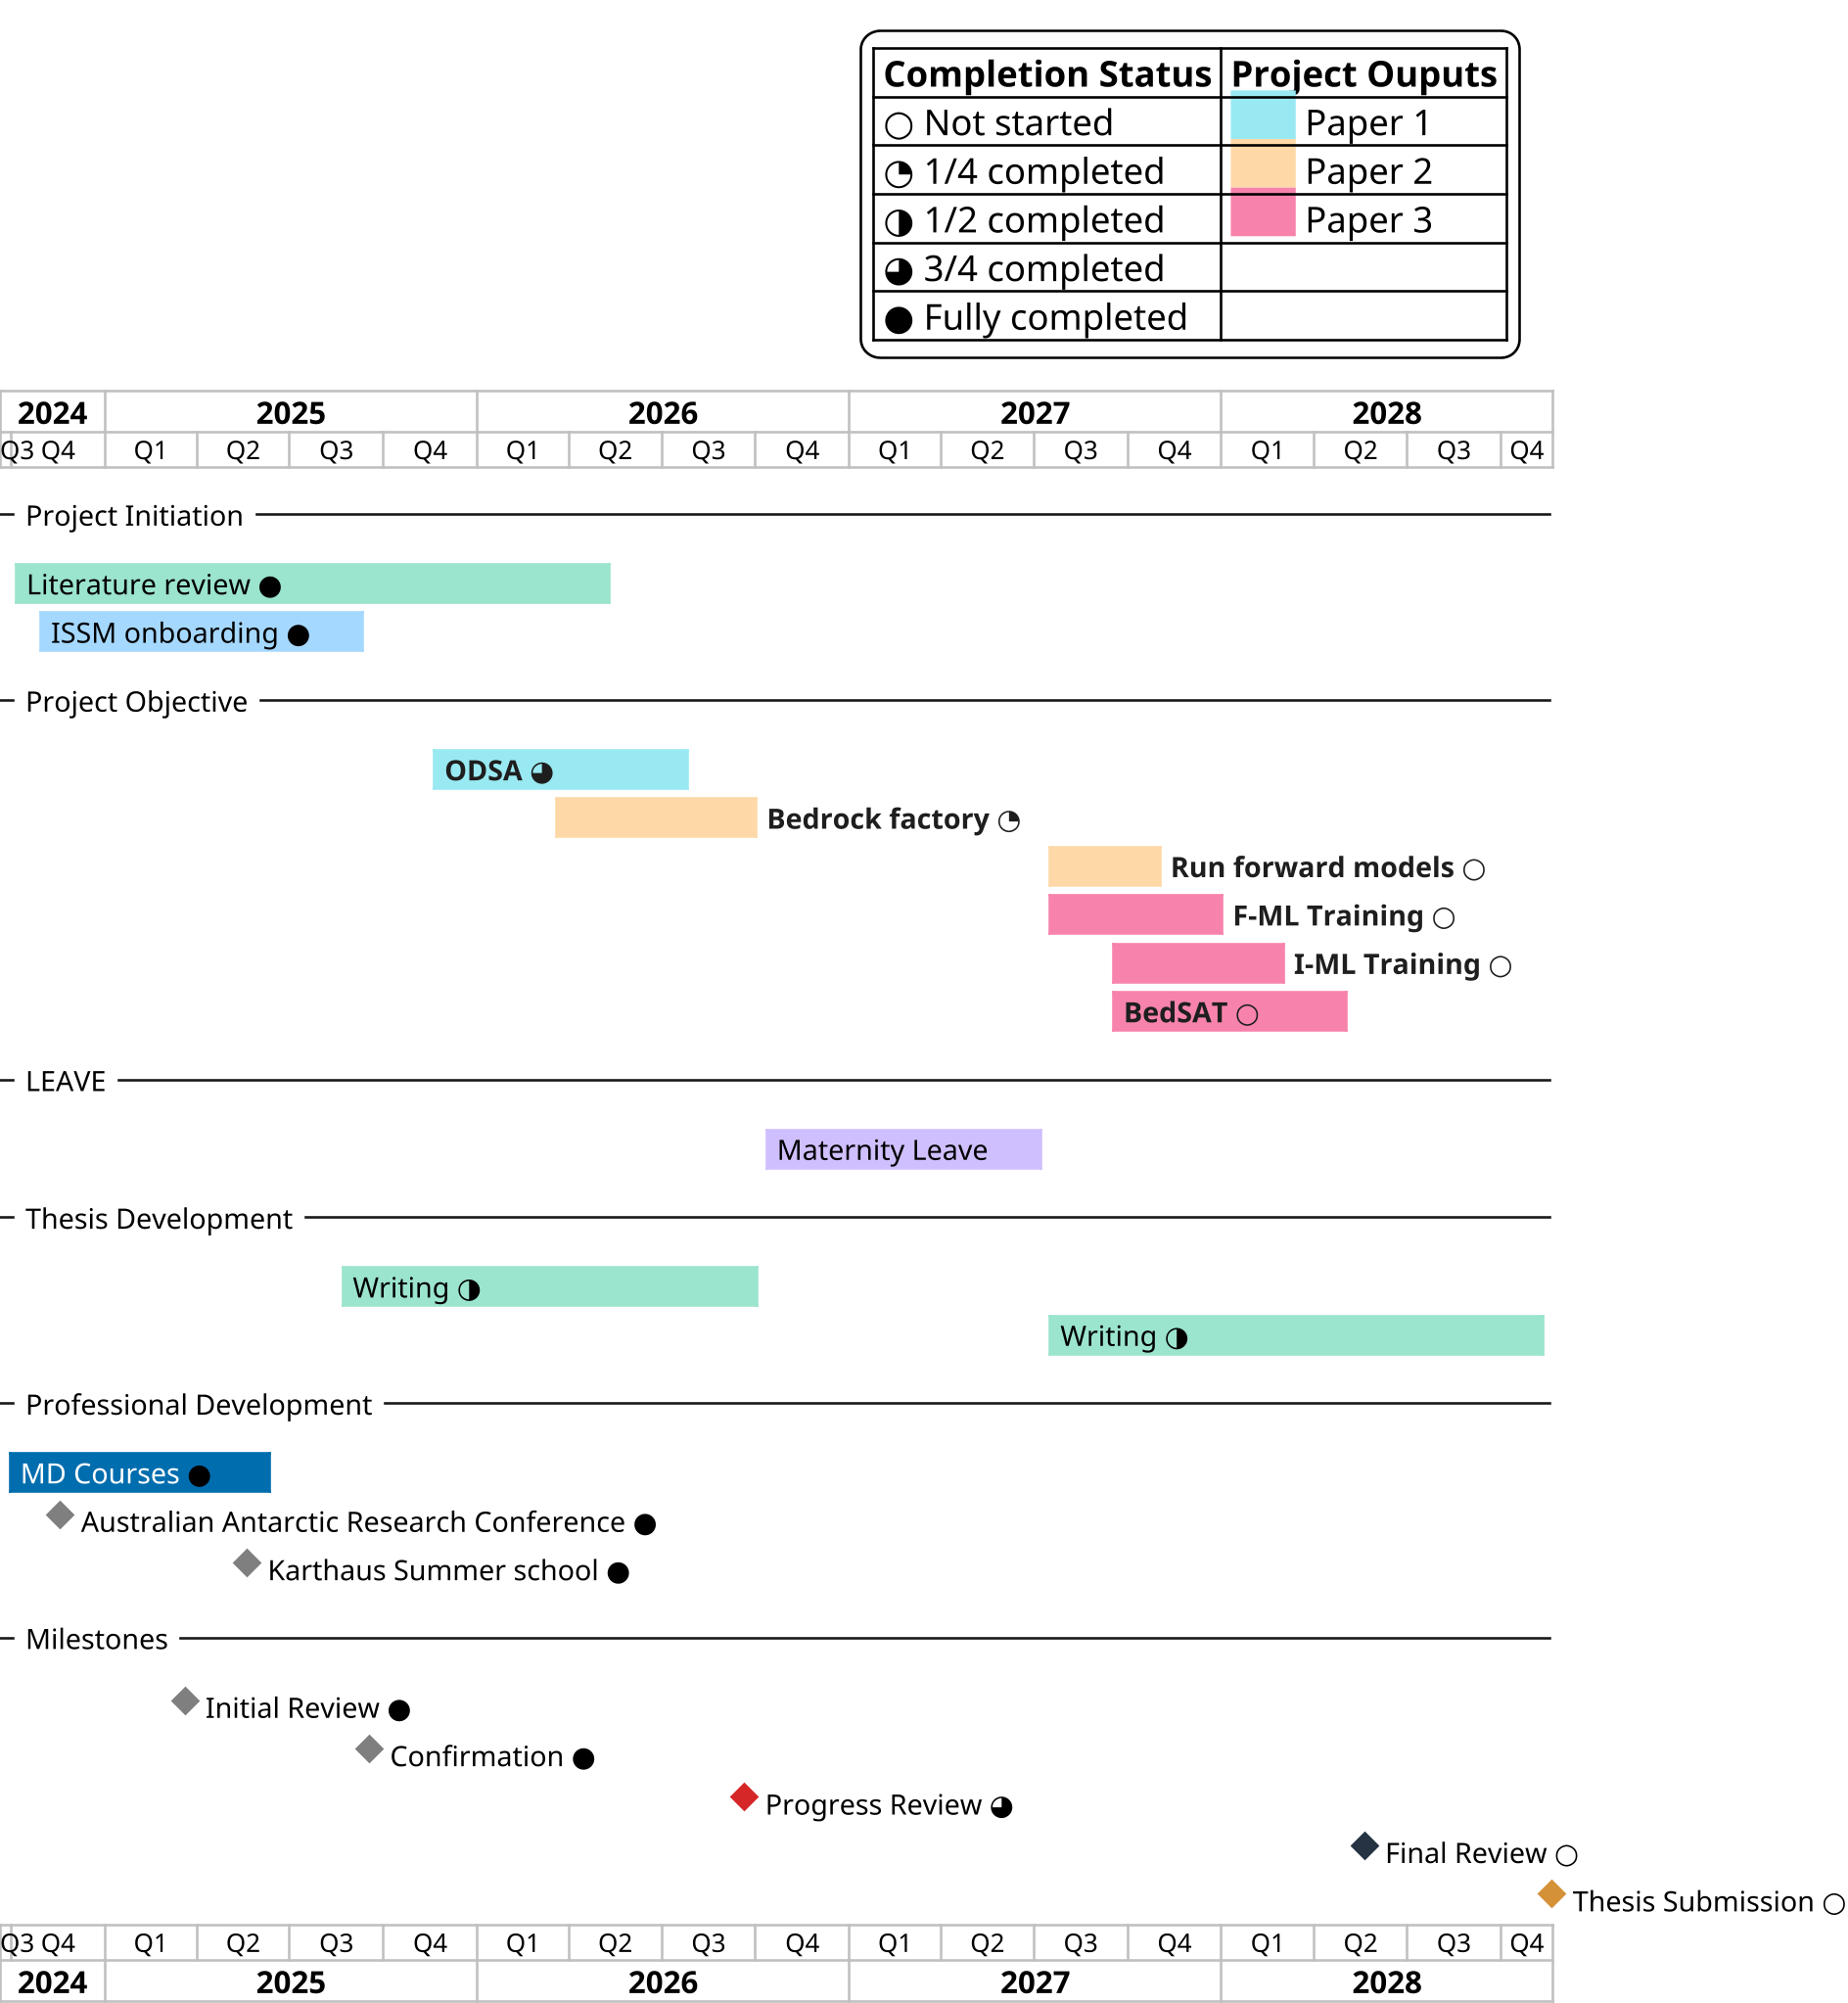
\includegraphics[width=1\linewidth]{figures/timeline.png}

%FMC: for the forward models, ML training, bedrock factory, do you have some of the workflow already? it might be worth describing, e.g., in a figure caption, what 1/4, 1/2, 3/4, means, particularly where you have already developed the code and workflow, but just need the inputs and to write the thing. 